\documentclass[a4paper,11pt]{article}

%%%%%%%%%%%%%%%%%%%%%%%%%%%%%%%%%%%%%%%%%%%%%%%%%%%%%%%%%%%%%%%%%%%%%%%%
% Paquetes utilizados
%%%%%%%%%%%%%%%%%%%%%%%%%%%%%%%%%%%%%%%%%%%%%%%%%%%%%%%%%%%%%%%%%%%%%%%%

% Graficos complejos
\usepackage{graphicx}
\usepackage{caption}
\usepackage{subcaption}
\usepackage{placeins}

% Soporte para el lenguaje español
\usepackage{textcomp}
\usepackage[utf8]{inputenc}
\usepackage[T1]{fontenc}
\DeclareUnicodeCharacter{B0}{\textdegree}
\usepackage[spanish]{babel}

% Matematicos
\usepackage{amssymb,amsmath}

% Soporte para arrays y tabs y formatos de columna
\usepackage{array}

% Soporte para subrayado
\usepackage{ulem}

% Soporte para enumerados
\usepackage{enumerate}

% PDFs embebidos para el apendice
\usepackage{pdfpages}

% Soporte para warnings
\usepackage{fixltx2e}

% Soporte para headers y footers
\usepackage{fancyhdr}
\setlength{\headheight}{15.2pt}
\pagestyle{fancy}
\fancyhf{}
\lhead{(71.15) Modelos y Optimización II} 
\rhead{TP1 Teoría de Colas}
\cfoot{\thepage}

% Soporte para colores
\usepackage{color}
\definecolor{color01}{rgb}{0.40,0.40,0.40}

\newcommand{\tab}{\hspace{5mm}}

% Formato de parrafo
\setlength{\parskip}{1ex plus 0.5ex minus 0.2ex}

%%%%%%%%%%%%%%%%%%%%%%%%%%%%%%%%%%%%%%%%%%%%%%%%%%%%%%%%%%%%%%%%%%%%%%%%
% Titulo
%%%%%%%%%%%%%%%%%%%%%%%%%%%%%%%%%%%%%%%%%%%%%%%%%%%%%%%%%%%%%%%%%%%%%%%%
%
%% Titulo principal del documento.
%\title{\textbf{Trabajo Práctico 1: Colas}}
%
%% Informacion sobre los autores.
%\author{\\
%  Cesar Buffevant, \textit{P. 76.700}                              \\
%  \texttt{buffevant@gmail.com}                                     \\ [2.5ex]
%  Juan Pecora, \textit{P. ??.???}                                  \\
%  \texttt{jlopezpecora@gmail.com}                                  \\ [2.5ex]
%  Flavio Olivieri, \textit{P. ??.???}                              \\
%  \texttt{flavio.olivieri@gmail.com}                               \\ [2.5ex]
%  Sergio Matias Piano, \textit{P. 85.191}                          \\
%  \texttt{smpiano@gmail.com}                                       \\ [2.5ex]
%  Florencia Tristant, \textit{P. 89.762}                           \\
%  \texttt{flotristant@gmail.com}                                   \\ [2.5ex]
%  \normalsize{1er. Cuatrimestre de 2015}                           \\
%  \normalsize{71.15 Modelos y Optimización 2}                      \\
%  \normalsize{Facultad de Ingeniería, Universidad de Buenos Aires} \\
%}
%\date{}
%
%%%%%%%%%%%%%%%%%%%%%%%%%%%%%%%%%%%%%%%%%%%%%%%%%%%%%%%%%%%%%%%%%%%%%%%%%
%% Documento
%%%%%%%%%%%%%%%%%%%%%%%%%%%%%%%%%%%%%%%%%%%%%%%%%%%%%%%%%%%%%%%%%%%%%%%%%
%\begin{document}
%\thispagestyle{empty}
%\maketitle
%
%\clearpage
\begin{document}
\thispagestyle{empty}

\begin{titlepage}

\newcommand{\HRule}{\rule{\linewidth}{0.5mm}}
\newenvironment{bottompar}{\par\vspace*{\fill}}{\clearpage}

\center

\textsc{\LARGE Universidad de Buenos Aires}\\[0.5cm]
\textsc{\Large Facultad de Ingeniería}\\[1.5cm]


\includegraphics[scale=0.5]{../logo.png}\\[1cm]


\textsc{\large (71.15) Modelos y Optimización II}\\[0.25cm]
\HRule \\[0.4cm]
{\huge \bfseries Teoría de Colas}\\[0.4cm]
\HRule \\[0.5cm]

{\large \today}

\begin{bottompar}
\flushleft
Buffevant, Cesar \textit{(buffevant@gmail.com)}         - P. 76.700

Pecora, Juan \textit{(jlopezpecora@gmail.com)}          - P. 84.700

Olivieri, Flavio \textit{(flavio.olivieri@gmail.com)}   - P. ??.???

Piano, Sergio \textit{(smpiano@gmail.com)}              - P. 85.191

Tristant, Florencia \textit{(flotristant@gmail.com)}    - P. 89.762
\end{bottompar}

\end{titlepage}

% ----------------------------------------------------------------------
% Tabla de contenidos
% ----------------------------------------------------------------------
\tableofcontents
\clearpage

\part{Resolución de ejercicios}
\section{\textbf{Ejercicio 1}}

\baselineskip=13pt
En una sastrería hay una sección de arreglo y reforma de la ropa vendida a sus
clientes, que es atendida por un sastre. El número de clientes que requieren
arreglos arriban a dicha sección con una distribución de Poisson con una media
de 24 clientes por hora. Debido a que el servicio es gratuito, todos los
clientes están dispuestos a esperar el tiempo que sea necesario para poder
utilizarlo. El tiempo de atención es en promedio de 2 minutos por cliente,
siendo exponencial la distribución de los tiempos de servicio. Calcular:

\leftskip=36pt
\parindent=-18pt
\begin{enumerate}[a)]
  \item ¿Cual es en promedio, el número de clientes en la sección?

  \item ¿Cuánto tiempo permanece, en promedio, un cliente en la sección?

  \item ¿Cual es la probabilidad de que el sastre esté desocupado?

  \item ¿Cual es en promedio, el número de clientes que están esperando recibir
    el servicio?
\end{enumerate}

\vspace{13pt}
\leftskip=0pt
\parindent=0pt
\subsection{\textbf{Resolución}}

Como sistema se entiende toda la sección de arreglo y
reforma.

\vspace{5pt}
\subsubsection*{Hipótesis:}

Se verifican las hipótesis de un P/P/1. El enunciado dice explícitamente que
todos los clientes están dispuestos a esperar el tiempo que sea necesario, lo
cual se puede interpretar como una cola con capacidad infinita.

\begin{enumerate}[1.]
  \item Tipo de proceso de arribo de clientes responde a distribución Poisson.
  \item Tipo de proceso de servicio a los clientes en el sistema responde a
    distribución Poisson.
  \item Hay un único canal de atención.
  \item El sistema tiene capacidad infinita.
  \item La disciplina de atención es FIFO.
  \item La población es infinita.
  \item Se forma una única cola frente al canal.
  \item El sistema se encuentra en régimen estacionario.
  \item La población no presenta fenómeno de impaciencia.
\end{enumerate}

\vspace{13pt}
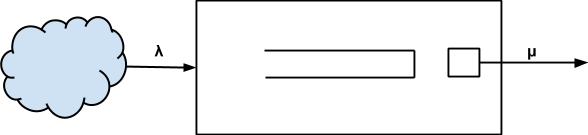
\includegraphics[width=341pt, height=101pt, keepaspectratio=true]{TP1-Colas-fig001.png}

\vspace{27pt}
Parámetros del modelo:

$\lambda = 24 [clientes/hora]$

$T_s = 2 [minutos/cliente] \times \frac{1[hora]}{60[minutos]} = 0.033
[horas/cliente]$ → $\mu = 30 [clientes/hora]$

\begin{enumerate}[a)]
  \vspace{13pt}
  \item El número de clientes en la sección, es decir el número de clientes en
    el sistema, es L.

  $L = \frac{\lambda}{\mu - \lambda} = \frac{24}{30 - 24} = 4 [clientes/hora]$

  \vspace{13pt}
  \item El tiempo que permanece un cliente en la sección, es decir, en el
    sistema es W:

  $W = \frac{1}{\mu-\lambda} = \frac{1}{30-24} = 0,1667[horas] \times \frac{60[minutos]}{1[hora]} = 10[minutos]$

  \vspace{13pt}
  \item La probabilidad de que el sastre esté desocupado es la probabilidad de
    que en la sección no haya nadie, es decir P(0)

  $P(0) = 1-\rho = 1-\frac{24}{30} = 0,2$

  \vspace{13pt}
  \item El número de clientes esperando recibir el servicio son los clientes
    que están en la cola, es decir $L_c$.

  $L_c = \frac{\rho^2}{1-\rho} = \frac{0,64}{1-0,8} = 3,2$

\end{enumerate}
\vspace{35pt}
\section{\textbf{Ejercicio 2}}

Un establecimiento de reparaciones, atendido por un solo operario, recibe un
promedio de cuatro clientes por hora, los cuales traen pequeños aparatos para
reparar.  El mecanico los inspecciona para encontrar defectos y muy a menudo
puede arreglarlos de inmediato, o de otro modo emitir un diagnostico. En
promedio, todo le toma 6 minutos por aparato. Los arribos tienen una
distribución de de Poisson y el tiempo de servicio tiene una distribución
exponencial. Calcular:

\leftskip=36pt
\parindent=-18pt
\begin{enumerate}[a)]
  \item La probabilidad de que el taller esté vacío.
  \item La probabilidad de que tres clientes estén en el taller.
  \item La probabilidad de encontrar por lo menos un cliente en el taller.
  \item El número promedio de clientes en el taller.
  \item El tiempo promedio que un cliente debe permanecer en el taller.
  \item El número promedio de clientes que esperan ser atendidos.
  \item El tiempo promedio que un cliente debe esperar para ser atendido.
\end{enumerate}

\vspace{13pt}
\leftskip=0pt
\parindent=0pt
\subsection{\textbf{Resolución}}

Consideramos el sistema como el taller, con el operario incluido. El enunciado
no dice nada con respecto a la capacidad de la cola, por lo que entendemos que
hay suficiente lugar como para albergar a toda la gente que arribe. Responde al
modelo P/P/1

\vspace{5pt}
\subsubsection*{Hipótesis:}

\begin{enumerate}[1.]
  \item Tipo de proceso de arribo de clientes responde a distribución Poisson.
  \item Tipo de proceso de servicio a los clientes en el sistema responde a
    distribución Poisson.
  \item Hay un único canal de atención.
  \item El sistema tiene capacidad infinita.
  \item La disciplina de atención es FIFO.
  \item La población es infinita.
  \item Se forma una única cola frente al canal.
  \item El sistema se encuentra en régimen estacionario.
  \item La población no presenta fenómeno de impaciencia.
\end{enumerate}

\vspace{13pt}
Parámetros del modelo:

$\lambda = 4 [clientes/hora]$

$T_s = 6 [minutos/cliente] \times \frac{1[hora]}{60[minutos]} = 0,1
[horas/cliente]$ → $\mu = 10 [clientes/hora]$.

\begin{enumerate}[a)]
  \vspace{13pt}
  \item La probabilidad de que el taller esté vacío es la probabilidad de que
    no haya ningún cliente en el sistema, es decir $P(0)$.

  $P(0) = 1-\rho = 1-\frac{4}{10} = 0,6$

  \vspace{13pt}
  \item La probabilidad de que tres cliente estén en el sistema es

  $P(3) = \rho^3 (1-\rho) = 0,4^3 \times 0,6 = 0,0384$

  \item La probabilidad de encontrar por lo menos a un cliente es

  $P(n > 0) = 1 - P(0) = 1 - 0.6 = 0.4.$

  \vspace{13pt}
  \item El número promedio de clientes en el taller es el número promedio de
    clientes en el sistema, es decir L.

  $L = \frac{\rho}{1-\rho} = \frac{0,4}{1-0,4} = 0,667$

  \vspace{13pt}
  \item El tiempo promedio que un cliente debe permanecer en el taller es el
    tiempo que un cliente debe permanecer en el sistema, es decir W.

  $W = \frac{1}{\mu-\lambda} = \frac{1}{10-4} = 0,1667[horas/cliente] \times
  \frac{60[minutos]}{1[hora]} = 10[minutos/cliente] $

  \vspace{13pt}
  \item El número de clientes que esperan ser atendidos son los clientes
    esperando en la cola, es decir $L_c$.

  $L_c = \frac{\rho^2}{1-\rho} = \frac{0,16}{1-0,4} = 0,2667$

  \vspace{13pt}
  \item El tiempo promedio que un cliente tiene que esperar para ser atendido
    es el tiempo que pasa en la cola, es decir $W_c$.

    $W_c = \frac{\lambda}{\mu(\mu-\lambda)} = \frac{4}{10\times(10-4)} =
    0,0667[horas/cliente] \times \frac{60[minutos]}{1[hora]} =
    4[minutos/cliente]$

\end{enumerate}

\vspace{35pt}
\section{\textbf{Ejercicio 3}}

Un banco está desarrollando la prestación de un nuevo servicio, para lo cual ha
habilitado una ventanilla. Como el desarrollo del mismo está basado en una
campaña publicitaria que hace mención al mínimo tiempo de espera que se
requiere, el gerente de la sucursal ha decidido encarar el estudio científico
del problema a fin de no exponerse a un fracaso. Hasta ahora se cuenta con los
siguientes datos:

\leftskip=36pt
\parindent=-18pt
\begin{itemize}
  \item Lapso medio entre arribo de usuarios: 8 minutos (distribución
    exponencial)
  \item Tiempo medio de atención en ventanilla: 2 minutos (distribución
    exponencial).
\end{itemize}

\leftskip=0pt
\parindent=0pt
Determinar:

\leftskip=36pt
\parindent=-18pt
\begin{enumerate}[a)]
  \item La probabilidad de esperar.
  \item La longitud promedio de la cola.
  \item La velocidad promedio de arribos que haría que el tiempo de espera en
    la cola supere los 4 minutos.
\end{enumerate}

\vspace{13pt}
\leftskip=0pt
\parindent=0pt
\subsection{\textbf{Resolución}}

Consideramos el sistema como la ventanilla más la cola. El enunciado no dice
nada con respecto a la capacidad de la cola, por lo que entendemos que hay
suficiente lugar como para albergar a toda la gente que arribe.

\vspace{5pt}
\subsubsection*{Hipótesis:}

Se verifican las hipótesis de un P/P/1.

\begin{enumerate}[1.]
  \item Tipo de proceso de arribo de clientes responde a distribución Poisson.
  \item Tipo de proceso de servicio a los clientes en el sistema responde a
    distribución Poisson.
  \item Hay un único canal de atención.
  \item El sistema tiene capacidad infinita.
  \item La disciplina de atención es FIFO.
  \item La población es infinita.
  \item Se forma una única cola frente al canal.
  \item El sistema se encuentra en régimen estacionario.
  \item La población no presenta fenómeno de impaciencia.
\end{enumerate}

\vspace{13pt}
Parámetros del modelo:

$T = 8 [minutos/cliente]$ →  $\lambda = 0,125 [clientes/minuto]$.

$Ts = 2 [minutos/cliente]$ → $\mu = 0,5 [clientes/minuto]$.

\begin{enumerate}[a)]
  \vspace{13pt}
  \item La probabilidad de esperar es la probabilidad de que en el sistema haya
    algún cliente, es decir $P(n>0) = 1 - P(0)$.

  $P(n>0) = 1 - P(0) = 1-1+\rho = \frac{\lambda}{\mu} = \frac{0,125}{0,5} =
  0,25$

  \vspace{13pt}
  \item La longitud promedio de la cola es la cantidad de clientes en promedio
    esperando para ser atendidos, es decir $L_c$.

  $L_c = \frac{\lambda^2}{\mu(\mu-\lambda)} = \frac{0,125^2}{0,5 \times
  (0,5-0,125)} = 0,0833$

  \vspace{13pt}
  \item El tiempo de espera en la cola es $W_c$, es decir:

  $W_c = \frac{\lambda}{\mu(\mu-\lambda)} < 4 \implies \lambda < 4
  \mu(\mu-\lambda) \implies \lambda < 4 \mu^2-4\mu\lambda \implies \lambda +
  4\mu\lambda < 4 \mu^2 \implies \lambda(1 + 4\mu) < 4\mu^2 \implies \lambda <
  \frac{4\mu^2}{1+4\mu}$

  $\lambda < \frac{4\mu^2}{1+4\mu} = \frac{4\times0,5^2}{1+4\times0,5} =
  0,333[clientes/minuto]$
\end{enumerate}

\vspace{35pt}
\section{\textbf{Ejercicio 4}}

Teniendo en cuenta el ejercicio 2, considerar todas las suposiciones
anteriores, excepto que si hay tres clientes en el taller, cualquier otro
cliente que llegue se retirará.

Determinar entonces:

\leftskip=36pt
\parindent=-18pt
\begin{enumerate}[a)]
  \item La probabilidad de que el taller esté vacío.
  \item La probabilidad de que tres clientes estén en el taller.
  \item La probabilidad de encontrar por lo menos un cliente en el taller.
  \item El número promedio de clientes en el taller.
  \item El tiempo promedio que un cliente debe permanecer en el taller.
  \item El número promedio de clientes que esperan ser atendidos.
  \item El tiempo promedio que un cliente debe esperar para ser atendido.
  \item La cantidad promedio de clientes que se retiran sin ser atendidos.
\end{enumerate}

\vspace{13pt}
\leftskip=0pt
\parindent=0pt
\subsection{\textbf{Resolución}}

\vspace{5pt}
\leftskip=0pt
\parindent=0pt
\subsubsection*{Hipótesis:}

\leftskip=36pt
\parindent=-18pt
\begin{itemize}
  \item El proceso de llegada de los clientes responde a un proceso Poisson.
  \item El proceso de atención de los clientes responde a un proceso Poisson.
  \item La población es infinita
  \item Se forma una única cola frente al canal de atención.
  \item Existe un único canal de atención.
  \item La capacidad del sistema es infinita
  \item La atención de los clientes de la cola es FIFO
  \item El sistema se encuentra en condiciones estables.
  \item \textit{La población presenta el fenómeno de impaciencia.}
\end{itemize}

\vspace{21pt}
\leftskip=0pt
\parindent=0pt
\textit{Sistema}

El sistema se modela como un sistema $P/P/1$ con impaciencia:

\vspace{13pt}
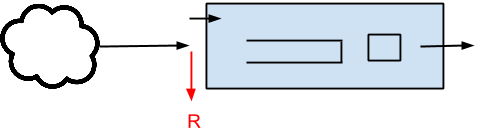
\includegraphics[width=359pt, height=99pt, keepaspectratio=true]{TP1-Colas-fig002.png}

$\lambda = 7,5[clientes/hora]$

$\mu = 30[clientes/hora]$


\vspace{27pt}
\begin{tabular}{|>{\centering}p{33pt}|>{\centering}p{31pt}|>{\centering}p{31pt}|>{\centering}p{31pt}|>{\centering}p{31pt}|>{\centering}p{31pt}|>{\centering}p{31pt}|>{\centering}p{31pt}|}
\hline
$n$ & $P(n)$ & $\lambda$ & $\mu$ & $L$ & $Lc$ & $H$ & $R$\tabularnewline
\hline
0 & $P(0)$ & $\lambda$ & 0 & 0 & 0 & 0 & 0\tabularnewline
\hline
1 & $P(1)$ & $\lambda$ & $\mu$ & 1 & 0 & 1 & 0\tabularnewline
\hline
2 & $P(2)$ & $\lambda$ & $\mu$ & 2 & 1 & 1 & 0\tabularnewline
\hline
3 & $P(3)$ & 0 & $\mu$ & 3 & 2 & 1 & $\lambda$\tabularnewline
\hline
4 & $P(4)$ & 0 & $\mu$ & 3 & 2 & 1 & $\lambda$\tabularnewline
\hline
5 & 0 & 0 & $\mu$ & 3 & 2 & 1 & $\lambda$\tabularnewline
\hline
.. & .. & ... & ... & ... & ... & ... & ...\tabularnewline
\hline
\end{tabular}

\vspace{13pt}
\leftskip=36pt
\parindent=-18pt
\begin{enumerate}[a)]
  \item 
    $P(1) = \frac{\lambda P(0)}{\mu} = \rho P(0)$ 

    $P(2) = \frac{\lambda P(1)}{\mu} = \rho^2P(0)$ 

    $P(3) = \frac{\lambda P(2)}{\mu} = \rho^3P(0)$ 

    $\rho = \frac{\lambda}{\mu} = \frac{7,5[clientes/hora]}{30[clientes/hora]}
    = 0,25$

    $P(0) + P(1) + P(2) +P(3) = 1 \implies P(0) =
    \frac{1}{1+\rho+\rho^2+\rho^3} = 0,75$
   

  \vspace{13pt}
  \item
    $P(3) = \rho^3P(0) = 0,012$ 

  \vspace{13pt}
  \item
    $1-P(0) = 1-0,75 = 0,25$ 

  \vspace{13pt}
  \item
    $L = 1 \times P(1) + 2 \times P(2) + 3 \times P(3) = 0,75
    \times(\rho+2\rho^2+3\rho^3) = 0,32$ 

  \vspace{13pt}
  \item
    $H = P(1) + P(2) + P(3) = 1 - P(0) = 0,25$ 

    $L_c = L - H = 0,52 - 0,25 = 0,27$ 

    $\lambda = \lambda(P(0) + P(1) + P(2)) = \lambda(1-P(3)) = \lambda(1-0,012)
    = 7,41 [clientes/hora]$ 

    $W = W_c + T_s = \frac{L_c}{\lambda} + \frac{1}{\mu} =
    \frac{0,27}{7,41[clientes/hora]} + \frac{1}{30[clientes/hora]} =
    0,069[horas/cliente] \times \frac{60[minutos]}{1[hora]} =
    4,18[minutos/cliente]$

  \vspace{13pt}
  \item
    $L_c = 0,27$

  \vspace{13pt}
  \item
    $\overline{\lambda} = \lambda(P(0) + P(1) + P(2)) = \lambda(1-P(3)) =
    \lambda(1-0,012) = 7,41[clientes/hora]$

    $W_c = \frac{L_c}{\lambda} = \frac{0,27}{7,41[clientes/hora]} =
    0,036[horas/cliente] \times \frac{60[minutos]}{1[hora]} =
    2,18[minutos/cliente]$

  \vspace{13pt}
  \item
    $R = \lambda P(3) = 0,09[clientes/hora]$
\end{enumerate}

\vspace{35pt}
\leftskip=0pt
\parindent=0pt
\section{\textbf{Ejercicio 5}}

Una empresa tiene cuatro máquinas cortadoras de césped. Las mismas se rompen o
necesitan mantenimiento cada 15 días (distribución exponencial). Para su
atención y mantenimiento tiene un empleado que en promedio tarda 7 días con
cada máquina. En promedio, por cada día de trabajo, las máquinas reportan un
ingreso de \$50. Se desea saber:
\begin{enumerate}[a)]
  \item El número promedio de máquinas funcionando.
  \item El porcentaje de tiempo que el empleado se encuentra inactivo.
  \item Cuánto tiempo, en promedio, estará en funcionamiento una máquina.
  \item Existe la posibilidad de contratar una persona más, que cobra 700\$ por
    mes y que tarda lo mismo que el empleado. Considerando 1 mes = 24 días,
    ¿conviene contratar al nuevo empleado?
\end{enumerate}


\vspace{13pt}
\leftskip=0pt
\parindent=0pt
\subsection{\textbf{Resolución}}

\vspace{21pt}
\subsubsection*{Hipótesis}

\leftskip=36pt
\parindent=-18pt
\begin{enumerate}[1.]
  \item El proceso de llegada de los clientes responde a un proceso Poisson.
  \item El proceso de atención de los clientes responde a un proceso Poisson.
  \item La población es infinita
  \item Se forma una única cola frente al canal de atención.
  \item Existe un único canal de atención.
  \item La capacidad del sistema es \textit{finita}
  \item La atención de los clientes de la cola es FIFO
  \item El sistema se encuentra en condiciones estables.
  \item La población no presenta el fenómeno de impaciencia.
\end{enumerate}

\vspace{21pt}
\leftskip=0pt
\parindent=0pt
\textit{Sistema}

El problema es un modelo de población finita:  $P/P/1/(N')$ con $N'=4$

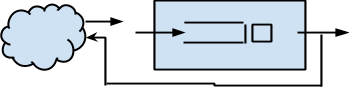
\includegraphics[width=262pt, height=67pt, keepaspectratio=true]{TP1-Colas-fig003.png}

$T_r = 15[dias]$

\vspace{27pt}
\begin{tabular}{|>{\centering}p{28pt}|>{\centering}p{26pt}|>{\centering}p{26pt}|>{\centering}p{26pt}|>{\centering}p{26pt}|>{\centering}p{26pt}|>{\centering}p{26pt}|>{\centering}p{26pt}|>{\centering}p{26pt}|}
\hline
$n$ & $P(n)$ & $\lambda$ & $\mu$ & $L$ & $Lc$ & $J$ & $N'$ & $H$\tabularnewline
\hline
0 & $P(0)$ & $4\lambda_R$ & 0 & 0 & 0 & 4 & 4 & 0\tabularnewline
\hline
1 & $P(1)$ & $3\lambda_R$ & $\mu$  & 1 & 0 & 3 & 4 & 1\tabularnewline
\hline
2 & $P(2)$ & $2\lambda_R$ & $\mu$  & 2 & 1 & 2 & 4 & 1\tabularnewline
\hline
3 & $P(3)$ & $\lambda_R$ & $\mu$  & 3 & 2 & 1 & 4 & 1\tabularnewline
\hline
4 & $P(4)$ & 0 &  & 4 & 3 & 0 & 4 & 1\tabularnewline
\hline
.. & 0 & .. & .. & .. & .. & .. & .. & ..\tabularnewline
\hline
\end{tabular}

\vspace{13pt}
\leftskip=36pt
\parindent=-18pt
\begin{enumerate}[a)]
  \item
    $J = 4P(0) + 3P(1) + 2P(2) + 1P(3)$

    $P(1) = \frac{4\lambda_R P(0)}{\mu} = 4\rho_R P(0)$

    $P(2) = \frac{3\lambda_R P(1)}{\mu} = 12\rho_R^2 P(0)$

    $P(3) = \frac{2\lambda_R P(2)}{\mu} = 24\rho_R^3 P(0)$

    $P(4) = \frac{\lambda_R P(3)}{\mu} = 24\rho_R^4 P(0)$

    $\rho_R = \frac{\lambda_R}{\mu} = \frac{\frac{1}{15}[clientes/dia]}{\frac{1}{7}[clientes/dia]} = \frac{7}{15}$

    $P(0) + P(1) + P(2) +P(3) = 1 \implies P(0) =
    \frac{1}{1+4\rho_R+12\rho_R^2+24\rho_R^3+24\rho_R^4} = 0,1241$

    $J = 2,1427$

  \vspace{13pt}
  \item
    $P(0) = 0,1241$

  \vspace{13pt}
  \item \textit{Estará en funcionamiento una sóla máquina cuando en el sistema haya 3 máquinas.}

    $P(3) = 24\rho_R^3 P(0) = 0,3027$

  \vspace{13pt}
  \item Para saber si conviene contratar un nuevo empleado a \$700 por mes, se
    plantea un nuevo sistema con 2 canales: $P/P/M/N$:

    \vspace{21pt}
    \leftskip=0pt
    \parindent=0pt
    \textit{Hipótesis}

    \leftskip=36pt
    \parindent=-18pt
    \begin{enumerate}[1.]
      \item El proceso de llegada de los clientes responde a un proceso Poisson.
      \item El proceso de atención de los clientes responde a un proceso Poisson.
      \item La población es infinita
      \item Se forma una única cola frente al canal de atención.
      \item \textit{Hay dos canales de atención}
      \item La capacidad del sistema es \textit{finita}
      \item La atención de los clientes de la cola es FIFO
      \item El sistema se encuentra en condiciones estables.
      \item La población no presenta el fenómeno de impaciencia.
    \end{enumerate}

    \vspace{21pt}
    \leftskip=0pt
    \parindent=0pt
    \textit{Modelo}

    Este problema es un modelo de población finita:  $P/P/1/(N')$ con $N'=4$

    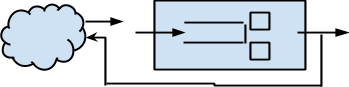
\includegraphics[width=262pt, height=67pt, keepaspectratio=true]{TP1-Colas-fig004.png}

    \vspace{55pt}
    \begin{tabular}{|>{\raggedright}p{28pt}|>{\raggedright}p{26pt}|>{\raggedright}p{26pt}|>{\raggedright}p{26pt}|>{\raggedright}p{26pt}|>{\raggedright}p{26pt}|>{\raggedright}p{26pt}|>{\raggedright}p{26pt}|>{\raggedright}p{26pt}|}
    \hline
    $n$ & $P(n)$ & $\lambda$ & $\mu$ & $L$ & $Lc$ & $J$ & $N'$ & $H$\tabularnewline
    \hline
    0 & $P(0)$ & $4\lambda_R$ & 0 & 0 & 0 & 4 & 4 & 0\tabularnewline
    \hline
    1 & $P(1)$ & $3\lambda_R$ & $\mu$ & 1 & 0 & 3 & 4 & 1\tabularnewline
    \hline
    2 & $P(2)$ & $2\lambda_R$ & 2$\mu$ & 2 & 1 & 2 & 4 & 1\tabularnewline
    \hline
    3 & $P(3)$ & $\lambda_R$ & 2$\mu$ & 3 & 2 & 1 & 4 & 1\tabularnewline
    \hline
    4 & $P(4)$ & 0 & 2$\mu$ & 4 & 3 & 0 & 4 & 1\tabularnewline
    \hline
    .. & 0 & .. & .. & .. & .. & .. & .. & ..\tabularnewline
    \hline
    \end{tabular}

    \vspace{13pt}
    $J = 4P(0) + 3P(1) + 2P(2) + 1P(3)$

    $P(1) = \frac{4\lambda_R P(0)}{\mu} = 4\rho_R P(0)$

    $P(2) = \frac{3\lambda_R P(1)}{2\mu} = 6\rho_R^2 P(0)$

    $P(3) = \frac{2\lambda_R P(2)}{2\mu} = 6\rho_R^3 P(0)$

    $P(4) = \frac{\lambda_R P(3)}{2\mu} = 3\rho_R^4 P(0)$

    $\rho_R = \frac{\lambda_R}{\mu} = \frac{\frac{1}{15}[clientes/dia]}{\frac{1}{7}[clientes/dia]} = \frac{7}{15}$

    $P(0) + P(1) + P(2) +P(3) = 1 \implies P(0) =
    \frac{1}{1+4\rho_R+12\rho_R^2+24\rho_R^3+24\rho_R^4} = 0,2548$

    $J = 3,2673$

    $I = \$50 \times 24[dias] \times J$

    Antes:

    $I = \$50 \times 24[dias] \times J = \$50[maquinas/dia] \times 24[dias] \times 2,1427 = \$2571,24[maquina]$

    Ahora:

    $I = \$50 \times 24[dias] \times J = \$50[maquinas/dia] \times 24[dias] \times 3,2673 = \$3920,76[maquina]$

    $Ganancia = \$3920,76[maquina] - \$2571,24[maquina] = \$1349,52[maquina] \implies Conviene $
\end{enumerate}

\vspace{35pt}
\leftskip=0pt
\parindent=0pt
\section{\textbf{Ejercicio 6}}

Una peluquería tiene un peluquero que realiza un corte de pelo especial a los
clientes. Recientemente se ha contratado un aprendiz para que lo ayude,
decidiendo que solo realice el corte cuando llega el segundo cliente a la cola
de espera.  Tanto el peluquero como el aprendiz demoran en promedio media hora
cada uno para atender a cada cliente. Al local llegan en promedio 5 clientes
por hora (distribución Poisson). Los clientes son impacientes. Si hay un
cliente esperando, solamente el 50\% de los clientes que llegan deciden entrar
a la peluquería. Si hay más de un cliente esperando, no entra ningún cliente
más ya que no están dispuestos a esperar. Se pide calcular: 

\begin{enumerate}[a)]
  \item La probabilidad de que no haya clientes en la peluquería. 
  \item La probabilidad de que haya clientes esperando para recibir el
    servicio. 
  \item El porcentaje de ocupación del peluquero y del aprendiz. 
  \item La cantidad promedio de clientes esperando para recibir el servicio. 
  \item La cantidad promedio de clientes que no ingresan a la peluquería. 
  \item Si cada corte de pelo cuesta 30\$, calcular el ingreso económico
    promedio de la peluquería, por hora.
\end{enumerate}


\vspace{13pt}
\leftskip=0pt
\parindent=0pt
\subsection{\textbf{Resolución}}


\vspace{13pt}
\textit{Modelo}

\vspace{13pt}
Este problema es un modelo $P/P/2$ con \textit{impaciencia}.

\vspace{13pt}
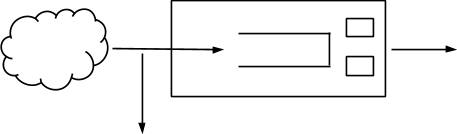
\includegraphics[width=343pt, height=102pt, keepaspectratio=true]{TP1-Colas-fig005.png}

\vspace{21pt}
\subsubsection*{Hipótesis}

\leftskip=36pt
\parindent=-18pt
\begin{enumerate}[1.]
  \item El proceso de llegada de los clientes responde a un proceso Poisson.
  \item El proceso de atención de los clientes responde a un proceso Poisson.
  \item La población es infinita
  \item Existen 2 canales de atención.
  \item Se forma una única cola frente a los canales de atención.
  \item La capacidad del sistema es in\textit{finita}
  \item La atención de los clientes de la cola es FIFO
  \item El sistema se encuentra en condiciones estables.
  \item La población presenta el fenómeno de impaciencia.
\end{enumerate}

\vspace{13pt}
\leftskip=0pt
\parindent=0pt
\textit{Datos}

\leftskip=36pt
\parindent=-18pt
\begin{enumerate}[a)]
  \item
    $\lambda = \frac{5[clientes]}{60[minuto]}$

  \item
    $\mu = \frac{1[cliente]}{60[minutos]}$

  \item Probabilidad de ingreso

    \leftskip=72pt
    \begin{enumerate}[1)]
      \item $n = 0 -> PI = 1$
      \item $n = 1 -> PI = 1$
      \item $n = 2 -> PI = 0.5$
      \item $n = 3 -> PI = 0.5$
      \item $n = 4 -> PI = 1$
    \end{enumerate}
\end{enumerate}

\vspace{13pt}
\begin{tabular}{|>{\centering}p{21pt}|>{\centering}p{24pt}|>{\centering}p{28pt}|>{\centering}p{28pt}|>{\centering}p{28pt}|>{\centering}p{19pt}|>{\centering}p{21pt}|>{\centering}p{21pt}|>{\centering}p{19pt}|>{\centering}p{19pt}|}
\hline
\centering $n$ & \centering $P(n)$ & \centering $\lambda$ & \centering $\mu$ & \centering $L$ & \centering $L_c$ & \centering $H$ & \centering $R$ & \centering $H1$ & \centering $H2$\tabularnewline
\hline
\centering 0 & $P(0)$ & $\lambda$ & \centering 0 & \centering 0 & \centering 0 & \centering 0 & \centering 0 & \centering 0 & \centering 0\tabularnewline
\hline
\centering 1 & $P(1)$ & $\lambda$ & \centering $\mu$ & \centering 1 & \centering 0 & \centering 1 & \centering 0 & \centering 1 & \centering 0\tabularnewline
\hline
\centering 2 & $P(2)$ & 0.5$\lambda$ & \centering $\mu$ & \centering 2 & \centering 1 & \centering 1 & \centering 0.5$\lambda$ & \centering 1 & \centering 0\tabularnewline
\hline
\centering 3 & $P(3)$ & 0.5$\lambda$ & \centering 2$\mu$ & \centering 3 & \centering 1 & \centering 2 & \centering 0.5$\lambda$ & \centering 1 & \centering 1\tabularnewline
\hline
\centering 4 & $P(4)$ & 0 & 2$\mu$ & \centering 4 & \centering 2 & \centering 2 & \centering $\lambda$ & \centering 1 & \centering 1\tabularnewline
\hline
\end{tabular}

\vspace{23pt}

$P(1) = \frac{\lambda P(0)}{\mu} \implies P(1) = \rho P(0) = 0,1553$

$P(2) = \frac{\lambda P(1)}{\mu} \implies P(2) = \rho^2 P(0) = 0,3882$

$P(3) = \frac{0,5\lambda P(2)}{2\mu} \implies P(3)= \frac{1}{4}\rho^3 P(0) = 0,2427$

$P(4) = \frac{0,5\lambda P(3)}{2\mu} \implies P(4) = \frac{1}{16}\rho^4 P(0) = 01517$

$P(0) + P(1) + P(2) + P(3) + P(4) = 1 \implies P(0) + \rho P(0) +  \rho^2 P(0) + \frac{1}{4}\rho^3 P(0) + \frac{1}{16}\rho^4 P(0) = 1$

$P(0) = \frac{1}{1 + \rho + \rho^2 + \frac{1}{4}\rho^3 + \frac{1}{16}\rho^4 } = 0,0621$

\vspace{27pt}
\begin{enumerate}[a)]
  \item Probabilidad de que no haya clientes en la peluquería.

  $P(0) = 0.0621$

  \vspace{13pt}
  \item Probabilidad de que haya clientes esperando para recibir el servicio.

  $P(2<n<4) = 0,7826$

  \vspace{13pt}
  \item Porcentaje de ocupación del peluquero y del aprendiz.

  $\overline{H_1} = \displaystyle\sum_{i=0}^{4} P(i) \times H_{1n} = 0,9379 \implies 93,97\% $

  $\overline{H_2} = \displaystyle\sum_{i=0}^{4} P(i) \times H_{2n} = 0,3944 \implies 39,44\% $

  \vspace{13pt}
  \parindent=0pt
  \item Cantidad promedio de clientes esperando para recibir el servicio.

  $\overline{L_c} = \displaystyle\sum_{i=0}^{4} P(i) \times L_{c_n} = 0,9343$

  \vspace{13pt}
  \item Cantidad promedio de clientes que no ingresan a la peluquería.

  $\overline{R} = \displaystyle\sum_{i=0}^{4} P(i) \times R_n = 2,3357[clientes/minuto]$

  \vspace{13pt}
  \item Si cada corte de pelo cuesta 30\$, calcular el ingreso económico promedio
    de la peluquería

  $\overline{I} = \left[ \displaystyle\sum_{i=0}^{4} P(i) \times \mu_n \right] \times 60[minutos] \times \$30 = \$79,93[minutos]$

\end{enumerate}

\vspace{35pt}
\leftskip=0pt
\parindent=0pt
\section{\textbf{Ejercicio 7}}

Dado el siguiente sistema:

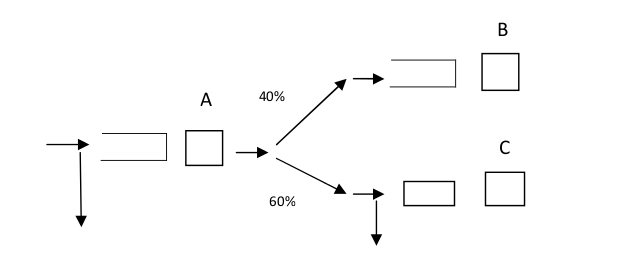
\includegraphics[width=316pt, height=141pt, keepaspectratio=true]{TP1-Colas-fig006.png}

\vspace{13pt}
Datos:
\begin{itemize}
  \item Arribos de clientes al sistema: 10 clientes/minuto
  \item Atención en cada canal:
    \begin{enumerate}[A:]
      \item 0,2 minutos/clientes
      \item 1/3 minutos/clientes                   
      \item 1/2 minutos/clientes
    \end{enumerate}

  \item Valor de cada servicio:
    \begin{enumerate}[A:]
      \item 0 \$/cliente     
      \item 5000 \$/cliente     
      \item 600 \$/cliente
    \end{enumerate}

  \item La población en el sector A es impaciente, según la siguiente ley:

  \vspace{13pt}
  \begin{tabular}{|>{\centering}p{28pt}|>{\centering}p{12pt}|>{\centering}p{18pt}|>{\centering}p{15pt}|>{\centering}p{9pt}|}
  \hline
  $n$ & 0 & 1 & 2 & 3\tabularnewline
  \hline
  $PI(n)$ & 1 & 0.5 & 0.2 & 0\tabularnewline
  \hline
  \end{tabular}
\end{itemize}

Se pide calcular:
\begin{enumerate}[a)]
  \item La cantidad promedio de clientes esperando en cada sector.
  \item El ingreso económico promedio del sistema (\$/minuto).
  \item La cantidad promedio de clientes que no ingresan al sistema por minuto.
  \item La probabilidad de que el sistema esté vacío.
\end{enumerate}

\vspace{13pt}
\leftskip=0pt
\parindent=0pt
\subsection{\textbf{Resolución}}

Como el sistema admite rechazo al ingreso del sistema y también para el caso de
la terminal C, se puede plantear el problema como 3 subsistemas independientes
y plantear que:

\vspace{13pt}
\parindent=0pt

$\lambda_{sistema} = \lambda_A = 10 [clientes/minuto]$

$\overline{\mu_{sistema}} = \overline{\mu_B} + \overline{\mu_C}$

$\overline{R_{sistema}} = \overline{R_A} + \overline{R_C}$

$\lambda_B = 0,4\overline{\mu_A}$

$\lambda_C = 0,6\overline{\mu_B}$

$T_{s_A} = 0,2 [minutos/cliente] \implies \mu_A = 5 [clientes/minuto]$

$T_{s_B} = \frac{1}{3} [minutos/cliente] \implies \mu_B = 3 [clientes/minuto]$

$T_{s_C} = \frac{1}{2} [minutos/cliente] \implies \mu_C = 2 [clientes/minuto]$


\vspace{69pt}
\subsubsection{Sistema A:}

\parindent=26pt
El sistema presenta las características de un modelo $P/P/1$ con impaciencia.

\vspace{5pt}
\parindent=26pt
\textit{Hipótesis}

\leftskip=36pt
\begin{itemize}
  \item El proceso de llegada de los clientes responde a un proceso Poisson.
  \item El proceso de atención de los clientes responde a un proceso Poisson.
  \item La población es infinita
  \item Se forma una única cola frente al canal de atención.
  \item Existe un único canal de atención.
  \item La capacidad del sistema es infinita
  \item La atención de los clientes de la cola es FIFO
  \item El sistema se encuentra en condiciones estables.
  \item \textit{La población presenta el fenómeno de impaciencia.}
\end{itemize}

\vspace{13pt}
\leftskip=0pt
\parindent=26pt
\begin{tabular}{|>{\centering}p{34pt}|>{\centering}p{33pt}|>{\centering}p{33pt}|>{\centering}p{33pt}|>{\centering}p{33pt}|>{\centering}p{33pt}|>{\centering}p{26pt}|>{\centering}p{27pt}|}
\hline
$n$ & $P(n)$ & $\lambda$ & $\mu$ & $L$ & $L_c$ & $H$ & $R$\tabularnewline
\hline
0 & $P(0)$ & $\lambda_A$ & 0 & 0 & 0 & 0 & 0\tabularnewline
\hline
1 & $P(1)$ & $0,5\lambda_A$ & $\mu_A$ & 1 & 0 & 1 & $0,5\lambda_A$\tabularnewline
\hline
2 & $P(2)$ & $0,2\lambda_A$ & $\mu_A$ & 2 & 1 & 1 & $0,8\lambda_A$\tabularnewline
\hline
3 & $P(3)$ & 0 & $\mu_A$ & 3 & 2 & 1 & $\mu_A$\tabularnewline
\hline
\end{tabular}

\vspace{13pt}
$P(1) = \frac{\lambda_A P(0)}{\mu_A} \implies P(1) = \rho_A P(0) = 0,3448$

$P(2) = \frac{0,5\lambda_A P(1)}{\mu_A} \implies P(2) = 0,5\rho_A^2 P(0) = 0,3448$

$P(3) = \frac{0,2\lambda_A P(2)}{\mu_A} \implies P(3) = 0,1\rho_A^3 P(0) = 0,13792$

$\rho_A = \frac{\lambda_A}{\mu_A} = \frac{10[clientes/minuto]}{5[clientes/minuto]} = 2$

$P(0) + P(1) + P(2) + P(3) = 1 \implies$

$P(0) + \rho_A P(0) +  0,5\rho_A^2 P(0) + 0,1\rho_A^3 P(0) = 1$

$P(0) = \frac{1}{1 + \rho_A + 0,5\rho_A^2 + 0,1\rho_A^3} = 0,1724$

$L_c = P(2) + 2P(3) = 0,3448 + 2 \times 0,13792 = 1,708$

$\overline{R_A} = 0,5\lambda_A P(1) + 0,8\lambda_A P(2) + \lambda_A P(3) = 2,9308$

$\overline{\mu_A} = \mu_A (P(1) + P(2) + P(3)) = \mu_A (1-P(0)) =$

$= 5[clientes/minuto]\times(1-0,1724) = 4,138[clientes/minuto]$


\vspace{27pt}
\subsubsection{Sistema B:}

\parindent=26pt
El sistema presenta las características de un modelo $P/P/1$.

\vspace{8pt}
\parindent=26pt
\textit{Hipótesis}

\leftskip=36pt
\parindent=-18pt
\begin{itemize}
  \item El proceso de llegada de los clientes responde a un proceso Poisson.
  \item El proceso de atención de los clientes responde a un proceso Poisson.
  \item La población es infinita
  \item Se forma una única cola frente al canal de atención.
  \item Existe un único canal de atención.
  \item La capacidad del sistema es infinita
  \item La atención de los clientes de la cola es FIFO
  \item El sistema se encuentra en condiciones estables.
  \item La población no presenta el fenómeno de impaciencia.
\end{itemize}

\vspace{27pt}
\leftskip=0pt
\parindent=26pt
\begin{tabular}{|>{\raggedright}p{39pt}|>{\raggedright}p{39pt}|>{\raggedright}p{38pt}|>{\raggedright}p{39pt}|>{\raggedright}p{38pt}|>{\raggedright}p{38pt}|>{\raggedright}p{31pt}|}
\hline
$n$ & $P(n)$ & $\lambda$ & $\mu$ & $L$ & $L_c$ & $H$\tabularnewline
\hline
0 & $P(0)$ & $\lambda_B$ & 0 & 0 & 0 & 0\tabularnewline
\hline
1 & $P(1)$ & $\lambda_B$ & $\mu_B$ & 1 & 0 & 1\tabularnewline
\hline
2 & $P(2)$ & $\lambda_B$ & $\mu_B$ & 2 & 1 & 1\tabularnewline
\hline
3 & $P(3)$ & $\lambda_B$ & $\mu_B$ & 3 & 2 & 1\tabularnewline
\hline
.... & .. & .. & .. & .. & .. & ..\tabularnewline
\hline
$n$ & $P(n)$ & $\lambda_B$ & $\mu_B$ & $n$ & $n-1$ & 1\tabularnewline
\hline       
\end{tabular}

\vspace{13pt}
$\lambda_B = 0,4\overline{\mu_B} = 0,4 \times 4,138[clientes/minuto] = 1,6552[clientes/minuto]$

$P(0) = 1-\rho_B = 1-\frac{\lambda_B}{\mu_B} = 1-0,5517 = 0,4483$

$\overline{\mu_B} = \overline{\lambda_B} = 1,6552[clientes/minuto]$

$L_c = \frac{\lambda_B}{\mu_B-\lambda_B} = \frac{1,6552[clientes/minuto]}{3[clientes/minuto]-1,6552[clientes/minuto]} = 1,2308$

$I = 5000[\$/cliente] \times \overline{\mu_B} = 5000[\$/cliente] \times 1,6552[clientes/minuto] =$

$= 8276[\$/minuto]$

\vspace{27pt}
\subsubsection{Sistema C:}

\parindent=26pt
Se trata de un sistema de capacidad limitada $P/P/1/N$ con $N=2$.

\vspace{8pt}
\parindent=26pt
\textit{Hipótesis}

\leftskip=36pt
\parindent=-18pt
\begin{itemize}
  \item El proceso de llegada de los clientes responde a un proceso Poisson.
  \item El proceso de atención de los clientes responde a un proceso Poisson.
  \item La población es infinita
  \item Se forma una única cola frente al canal de atención.
  \item Existe un único canal de atención.
  \item \textit{La capacidad del sistema es finita}
  \item La atención de los clientes de la cola es FIFO
  \item El sistema se encuentra en condiciones estables.
  \item La población no presenta el fenómeno de impaciencia.
\end{itemize}

\vspace{27pt}
\leftskip=0pt
\parindent=26pt
\begin{tabular}{|>{\centering}p{34pt}|>{\centering}p{33pt}|>{\centering}p{33pt}|>{\centering}p{33pt}|>{\centering}p{33pt}|>{\centering}p{33pt}|>{\centering}p{26pt}|>{\centering}p{27pt}|}
\hline
$n$ & $P(n)$ & $\lambda$ & $\mu$ & $L$ & $L_c$ & $H$ & $R$\tabularnewline
\hline
0 & $P(0)$ & $\lambda_C$ & 0 & 0 & 0 & 0 & 0\tabularnewline
\hline
1 & $P(1)$ & $\lambda_C$ & $\mu_C$ & 1 & 0 & 1 & 0\tabularnewline
\hline
2 & $P(2)$ & 0 & $\mu_C$ & 2 & 1 & 1 & $\lambda_C$\tabularnewline
\hline
\end{tabular}

\vspace{13pt}
$\lambda_C = 0,6\overline{\mu_C} = 0,6 \times 4,138[clientes/minuto] = 2,4828[clientes/minuto]$

$P(1) = \frac{\lambda_C P(0)}{\mu_C} \implies P(1) = \rho_C P(0) = 0,3281$

$P(2) = \frac{\lambda_C P(1)}{\mu_C} \implies P(2) = \rho_C^2 P(0) = 0,4075$

$\rho_C = \frac{\lambda_C}{\mu_C} = \frac{2,4828[clientes/minuto]}{2[clientes/minuto]} = 1,2414$

$P(0) + P(1) + P(2) = 1 \implies$

$P(0) + \rho_A P(0) +  \rho_C^2 P(0) = 1$

$P(0) = \frac{1}{1 + \rho_C + \rho_C^2} = 0,2644$

$\overline{\mu_C} = \mu_C \times P(1) + \mu_C \times P(2) = 2[clientes/minuto] \times(0,3281 + 0,4075) =$

$= 1,4712[clientes/minuto]$

$L_c = P(2) = 0,4075$

$R_C = \lambda_C \times P(2) = 2,4828[clientes/minuto] \times 0,4075 = 1,012[clientes/minuto]$

$I = 600[\$/cliente] \times \overline{\mu_C} = 600[\$/cliente] \times 1,4712[clientes/minuto] =$

$= 882,72[\$/minuto]$



\vspace{13pt}
\subsubsection{Conclusion:}

\leftskip=36pt
\parindent=-18pt
\begin{enumerate}[a)]
  \item La cantidad promedio de clientes esperando en cada sector.

    $L_{c_A} = 1,708$

    $L_{c_B} = 1,2308$

    $L_{c_C} = 1,4075$

  \vspace{13pt}
  \item El ingreso económico promedio del sistema (\$/minuto).

    $I = I_A + I_B + I_C = 0[\$/minuto] + 8276[\$/minuto] + 882,72[\$/minuto] = 9158,72[\$/minuto]$

  \vspace{13pt}
  \item La cantidad promedio de clientes que no ingresan al sistema por minuto.

    $R_{sistema} = R_A + R_C = 2,9308[clientes/minuto]  + 1,012[clientes/minuto] = 3,9425[clientes/minuto]$

  \vspace{13pt}
  \item La probabilidad de que el sistema esté vacío.

    $P(0) = P_A(0) \times P_B(0) \times P_C(0) = 0,1724 \times 0,4483 \times 0,2644 = 0,021$

\end{enumerate}

\vspace{35pt}
\leftskip=0pt
\parindent=0pt
\section{\textbf{Ejercicio 8}}

\vspace{13pt}
Dado el siguiente sistema con reciclaje:

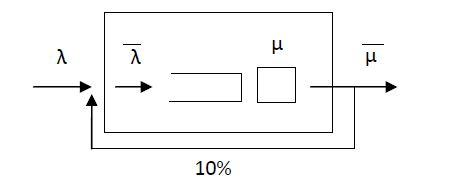
\includegraphics[width=338pt, height=141pt, keepaspectratio=true]{TP1-Colas-fig007.png}

\vspace{27pt}
Sabiendo que los clientes arriban a una velocidad promedio de 8 clientes por
minuto y el canal atiende a una velocidad promedio de 10 clientes por minuto
(distribución Poisson), se pide calcular:
\begin{enumerate}[a)]
  \item La cantidad promedio de clientes en la cola.
  \item El tiempo promedio de permanencia de un cliente en la cola.
  \item La probabilidad de que el canal no esté ocioso.
  \item La cantidad promedio de clientes en el sistema.
\end{enumerate}

\vspace{13pt}
\leftskip=0pt
\parindent=0pt
\subsection{\textbf{Resolución}}

Se usan fórmulas de P/P/1 pero con $\lambda$ esperado 
en vez de $\lambda$, por ser con reciclaje.

\vspace{21pt}
\subsubsection*{Hipótesis}

\leftskip=36pt
\parindent=-18pt
\begin{enumerate}[1.]
  \item El proceso de arribo de los clientes al sistema es Poisson.
  \item El proceso de servicio del canal es Poisson.
  \item El sistema se encuentra en régimen permanente.
  \item Los clientes que llegan al sistema forman una cola simple.
  \item La disciplina de atención es FIFO.
  \item Hay un solo canal de atención.
  \item La capacidad del sistema es infinita.
  \item Los clientes que llegan al sistema no presentan impaciencia.
  \item La población de potenciales clientes del sistema es infinita.
\end{enumerate}

\vspace{13pt}
\begin{enumerate}[a)]
  \item Cantidad promedio de clientes en la cola.

    $\overline{\lambda} = \lambda + 0,1\overline{\mu}$

  Y siendo: 

  $\overline{\lambda} = \overline{\mu} \implies \overline{\lambda} = \lambda + 0,1\overline{\lambda}$

  $0,9\overline{\lambda} = \lambda$

  Por lo que  

  $\overline{\lambda} = \frac{\lambda \times 10}{9} = \frac{8[clientes/minuto] \times 10}{9} =  8,88[clientes/minuto]$

  $\overline{\lambda} = \lambda_{esperado} =  8,88[clientes/minuto]$

  Siendo 

  $L_c = \left.\frac{\lambda^2}{\mu(\mu-\lambda)}\right|_{\lambda=\lambda_{esperado}} = \frac{\frac{80}{9}^2}{10 \times (10-\frac{80}{9}} = 7,11$

  \vspace{13pt}
  \item Tiempo promedio de permanencia de un cliente en la cola.

    $W_c = \left.\frac{L_c}{\lambda}\right|_{\lambda=\lambda_{esperado}} = \frac{\frac{64}{9}}{\frac{80}{9}} = 7,11$

  \vspace{13pt}
  \item Probabilidad de que el canal no esté ocioso.

  $P(n \geq 1) = 1-P(n=0) = 1-(1-\rho) = \rho = 0,88$

  Dado que:

  $\rho = \left.\frac{\lambda}{\mu}\right|_{\lambda=\lambda_{esperado}} = \frac{\frac{80}{9}}{10} = 0,88$

  \vspace{13pt}
  \item Cantidad promedio de clientes en el sistema.\label{h.8dp3y8yzivhk}

    $L = L_c + H = \frac{\lambda^2}{\mu(\mu-\lambda)} + \rho = \left.\frac{\lambda}{\mu-\lambda}\right|_{\lambda=\lambda_{esperado}} = \frac{\frac{80}{9}}{10 \times \frac{80}{9}}$

\end{enumerate}

\vspace{35pt}
\leftskip=0pt
\parindent=0pt
\section{\textbf{Ejercicio 9}}

\vspace{13pt}
Dado el siguiente sistema, los clientes que ingresan al mismo deben pasar por
dos sectores para realizar su trámite. En el primer sector se realiza la
primera parte del trámite.  Allí hay dos ventanillas, la 1 y la 2, que brindan
el mismo servicio, a una velocidad $\mu_1$ y $\mu_2$ respectivamente. La segunda
parte del trámite se lleva a cabo en el segundo sector, el cual cuenta con
otras dos ventanillas (la 3 y la 4), que atienden a una velocidad $\mu_3$ y
$\mu_4$ respectivamente.  Ambas brindan el mismo servicio. Dado que no hay mucho
espacio, no se admite formación de cola ni antes del primer sector ni antes del
segundo. Los clientes que ingresan al sistema no pueden retirarse sin haber
realizado el trámite completo.

\vspace{13pt}
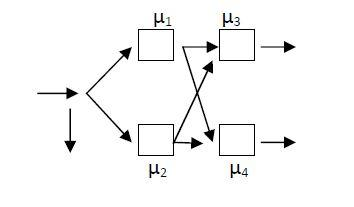
\includegraphics[width=266pt, height=155pt, keepaspectratio=true]{TP1-Colas-fig008.png}

\vspace{13pt}
Se pide:
\begin{enumerate}[a)]
  \item Definir todos los estados posibles.
  \item Expresar P(b,0,1,1)
  \item Expresar P(0,0,1,1)  
\end{enumerate}

\vspace{13pt}
\leftskip=0pt
\parindent=0pt
\subsection{\textbf{Resolución}}

\vspace{21pt}
\subsubsection*{Hipótesis}

\leftskip=36pt
\parindent=-18pt
\begin{enumerate}[1.]
  \item El proceso de arribo de los clientes al sistema es Poisson.
  \item El proceso de servicio del canal es Poisson.
  \item El sistema se encuentra en régimen permanente. 
  \item Los clientes que llegan al sistema forman una cola simple. 
  \item La disciplina de atención es FIFO. 
  \item La capacidad del sistema es infinita. 
  \item Los clientes que llegan al sistema no presentan impaciencia.
  \item La población es infinita.
  \item En ambas instancias los canales son indistintos para el cliente (no hay
    preferencia). 
  \item El cliente no conoce la velocidad de cada canal.
\end{enumerate}

\vspace{13pt}
\begin{enumerate}[a)]
  \item Definir todos los estados posibles

  \begin{tabular}{|>{\centering}p{22pt}|>{\centering}p{16pt}|>{\centering}p{15pt}|>{\centering}p{16pt}|>{\centering}p{15pt}|}
  \hline
  \centering n & \centering $C_1$ & \centering $C_2$ & \centering $C_3$ & \centering $C_4$\tabularnewline
  \hline
  \centering 0 & \centering 0 & \centering 0 & \centering 0 & \centering 0\tabularnewline
  \hline
  \centering 1 & \centering 1\linebreak{}
  0\linebreak{}
  0\linebreak{}
  0 & \centering 0\linebreak{}
  1\linebreak{}
  0\linebreak{}
  0 & \centering 0\linebreak{}
  0\linebreak{}
  1\linebreak{}
  0 & \centering 0\linebreak{}
  0\linebreak{}
  0\linebreak{}
  1\tabularnewline
  \hline
  \centering 2 & \centering 1\linebreak{}
  1\linebreak{}
  1\linebreak{}
  0\linebreak{}
  0\linebreak{}
  0 & \centering 1\linebreak{}
  0\linebreak{}
  0\linebreak{}
  1\linebreak{}
  1\linebreak{}
  0 & \centering 0\linebreak{}
  1\linebreak{}
  0\linebreak{}
  1\linebreak{}
  0\linebreak{}
  1 & \centering 0\linebreak{}
  0\linebreak{}
  1\linebreak{}
  0\linebreak{}
  1\linebreak{}
  1\tabularnewline
  \hline
  \centering 3 & \centering 1\linebreak{}
  1\linebreak{}
  1\linebreak{}
  0\linebreak{}
  b\linebreak{}
  0 & \centering 1\linebreak{}
  1\linebreak{}
  0\linebreak{}
  1\linebreak{}
  0\linebreak{}
  b & \centering 1\linebreak{}
  0\linebreak{}
  1\linebreak{}
  1\linebreak{}
  1\linebreak{}
  1 & \centering 0\linebreak{}
  1\linebreak{}
  1\linebreak{}
  1\linebreak{}
  1\linebreak{}
  1\tabularnewline
  \hline
  \centering 4 & \centering 1\linebreak{}
  b\linebreak{}
  b\linebreak{}
  1 & \centering 1\linebreak{}
  b\linebreak{}
  1\linebreak{}
  b & \centering 1\linebreak{}
  1\linebreak{}
  1\linebreak{}
  1 & \centering 1\linebreak{}
  1\linebreak{}
  1\linebreak{}
  1\tabularnewline
  \hline
  \end{tabular}


  \vspace{13pt}
  \item Expresar P(b,0,1,1)

  \leftskip=6pt
  \parindent=-18pt
  $P(b,0,1,1) = P(1,0,1,1) \times P(b,0,1,1) \times (1-\mu_3\Delta t) \times (1-\mu_4\Delta t) \times (1-\lambda\Delta t) +$
  $ P(b,0,1,1) \times \mu_1\Delta t \times (1-\mu_3\Delta t) \times (1-\mu_4\Delta t) \times (1-\lambda\Delta t) +$
  $ P(b,b,0,1) \times \mu_3\Delta t \times 0,5 \times (1-\mu_4\Delta t) +$
  $ P(b,b,0,1) \times \mu_4\Delta t \times 0,5 \times (1-\mu_3\Delta t) +$

  \vspace{13pt}
  \item Expresar P(0,0,1,1)

  \leftskip=6pt
  \parindent=-18pt
  $P(0,0,1,1) = P(1,0,1,1) \times (1-\mu_3\Delta t) \times (1-\mu_4\Delta t) \times (1-\lambda\Delta t) +$
  $ P(1,0,1,0) \times \mu_1\Delta t \times (1-\mu_3\Delta t) \times (1-\lambda\Delta t) +$
  $ P(1,0,0,1) \times \mu_1\Delta t \times (1-\mu_4\Delta t) \times (1-\lambda\Delta t) +$
  $ P(0,1,1,0) \times \mu_2\Delta t \times (1-\mu_3\Delta t) \times (1-\lambda\Delta t) +$
  $ P(0,1,0,1) \times \mu_2\Delta t \times (1-\mu_4\Delta t) \times (1-\lambda\Delta t) +$
  $ P(b,0,1,1) \times \mu_3\Delta t \times (1-\mu_4\Delta t) \times (1-\lambda\Delta t) +$
  $ P(b,0,1,1) \times \mu_4\Delta t \times (1-\mu_3\Delta t) \times (1-\lambda\Delta t) +$
  $ P(0,b,1,1) \times \mu_3\Delta t \times (1-\mu_4\Delta t) \times (1-\lambda\Delta t) +$
  $ P(0,b,1,1) \times \mu_4\Delta t \times (1-\mu_3\Delta t) \times (1-\lambda\Delta t)$

\end{enumerate}

\vspace{35pt}
\leftskip=0pt
\parindent=0pt
\section{\textbf{Ejercicio 10}}

Dado el siguiente sistema de atención al público:

\vspace{13pt}
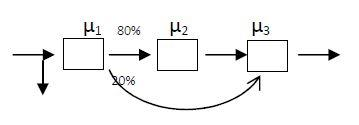
\includegraphics[width=269pt, height=94pt, keepaspectratio=true]{TP1-Colas-fig009.png}

\vspace{13pt}
Se sabe que, según el tipo de trámite, el 80\% de los clientes que salen del
canal 1 pasan directamente al canal 2, mientras que el 20\% restante pasa
directamente al canal 3. Las velocidades de atención de cada canal son $\mu_1$,
$\mu_2$ y $\mu_3$, respectivamente.  No se admite abandono: el cliente que
ingresa al sistema no sale del mismo sin haber recibido el servicio que allí se
brinda.
Debido a que el lugar es reducido, no se admite formación de cola
frente a ninguno de los canales.

Se pide expresar:

\begin{enumerate}[a)]
  \item Todos los posibles estados.
  \item Calcular P(0,1,1).
  \item Calcular P(1,0,1).
\end{enumerate}

\vspace{13pt}
\leftskip=0pt
\parindent=0pt
\subsection{\textbf{Resolución}}

\vspace{21pt}
\subsubsection*{Hipótesis}

\leftskip=36pt
\parindent=-18pt
\begin{enumerate}[1.]
  \item El proceso de arribo de los clientes al sistema es Poisson.
  \item El proceso de servicio del canal es Poisson.
  \item El sistema se encuentra en régimen permanente.
  \item Los clientes que llegan al sistema forman una cola simple.
  \item La disciplina de atención es FIFO.
  \item La capacidad del sistema es infinita.
  \item Los clientes que llegan al sistema no presentan impaciencia.
  \item La población es infinita. 
  \item Luego del canal 1 existe obligación, es decir los clientes deberán ir al
     canal 2 o 3 respectivamente (dependiendo del trámite).
\end{enumerate}

\vspace{13pt}
\begin{enumerate}[a)]
  \item Estados posibles

  \vspace{13pt}
  \leftskip=0pt
  \begin{tabular}{|>{\raggedright}p{22pt}|>{\raggedright}p{16pt}|>{\raggedright}p{15pt}|>{\raggedright}p{16pt}|}
  \hline
  \centering n & \centering $C_1$ & \centering $C_2$ & \centering $C_3$\tabularnewline
  \hline
  \centering 0 & \centering 0 & \centering 0 & \centering 0\tabularnewline
  \hline
  \centering 1 & \centering 1\linebreak{}
  0\linebreak{}
  0 & \centering 0\linebreak{}
  1\linebreak{}
  0 & \centering 0\linebreak{}
  0\linebreak{}
  1\tabularnewline
  \hline
  \centering 2 & \centering 0\linebreak{}
  1\linebreak{}
  1\linebreak{}
  b\linebreak{}
  b\linebreak{}
  0 & \centering 1\linebreak{}
  0\linebreak{}
  1\linebreak{}
  1\linebreak{}
  0\linebreak{}
  b & \centering 1\linebreak{}
  1\linebreak{}
  0\linebreak{}
  0\linebreak{}
  1\linebreak{}
  1\tabularnewline
  \hline
  \centering 3 & \centering 1\linebreak{}
  b\linebreak{}
  1\linebreak{}
  b & \centering 1\linebreak{}
  1\linebreak{}
  b\linebreak{}
  b & \centering 1\linebreak{}
  1\linebreak{}
  1\linebreak{}
  1\tabularnewline
  \hline
  \end{tabular}

  \vspace{13pt}
  \item Cálculo de P(0,1,1).

  $P(0,0,1) = P(1,1,0) \times \mu_1\Delta t \times 0,2 \times (1-\mu_2\Delta t) +$
  $P(1,0,1) \times \mu_1\Delta t \times 0,8 \times (1-\mu_3\Delta t) +$
  $P(0,1,1) \times \mu_2\Delta t \times (1-\lambda\Delta t) \times (1-\mu_3\Delta t) +$
  $P(b,1,0) \times \mu_2\Delta t +$
  $P(b,1,1) \times \mu_3\Delta t \times 0,2 \times (1-\mu_2\Delta t) +$
  $P(b,b,1) \times \mu_3\Delta t \times 0,8$

  \vspace{13pt}
  \item Cálculo de P(1,0,1).

  $P(1,0,1) = P(0,0,1) \times \lambda\Delta t \times (1-\mu_3\Delta t) +$
  $P(1,1,0) \times \mu_2\Delta t \times (1-\mu_1\Delta t) +$
  $P(1,0,1) \times (1-\mu_1\Delta t) \times (1-\mu_3\Delta t) +$
  $P(1,b,1) \times \mu_3\Delta t \times (1-\mu_1\Delta t)$

\end{enumerate}

\newpage

\part{Apéndice}
\appendix

\section{Enunciado original}\label{sec:enunciado}
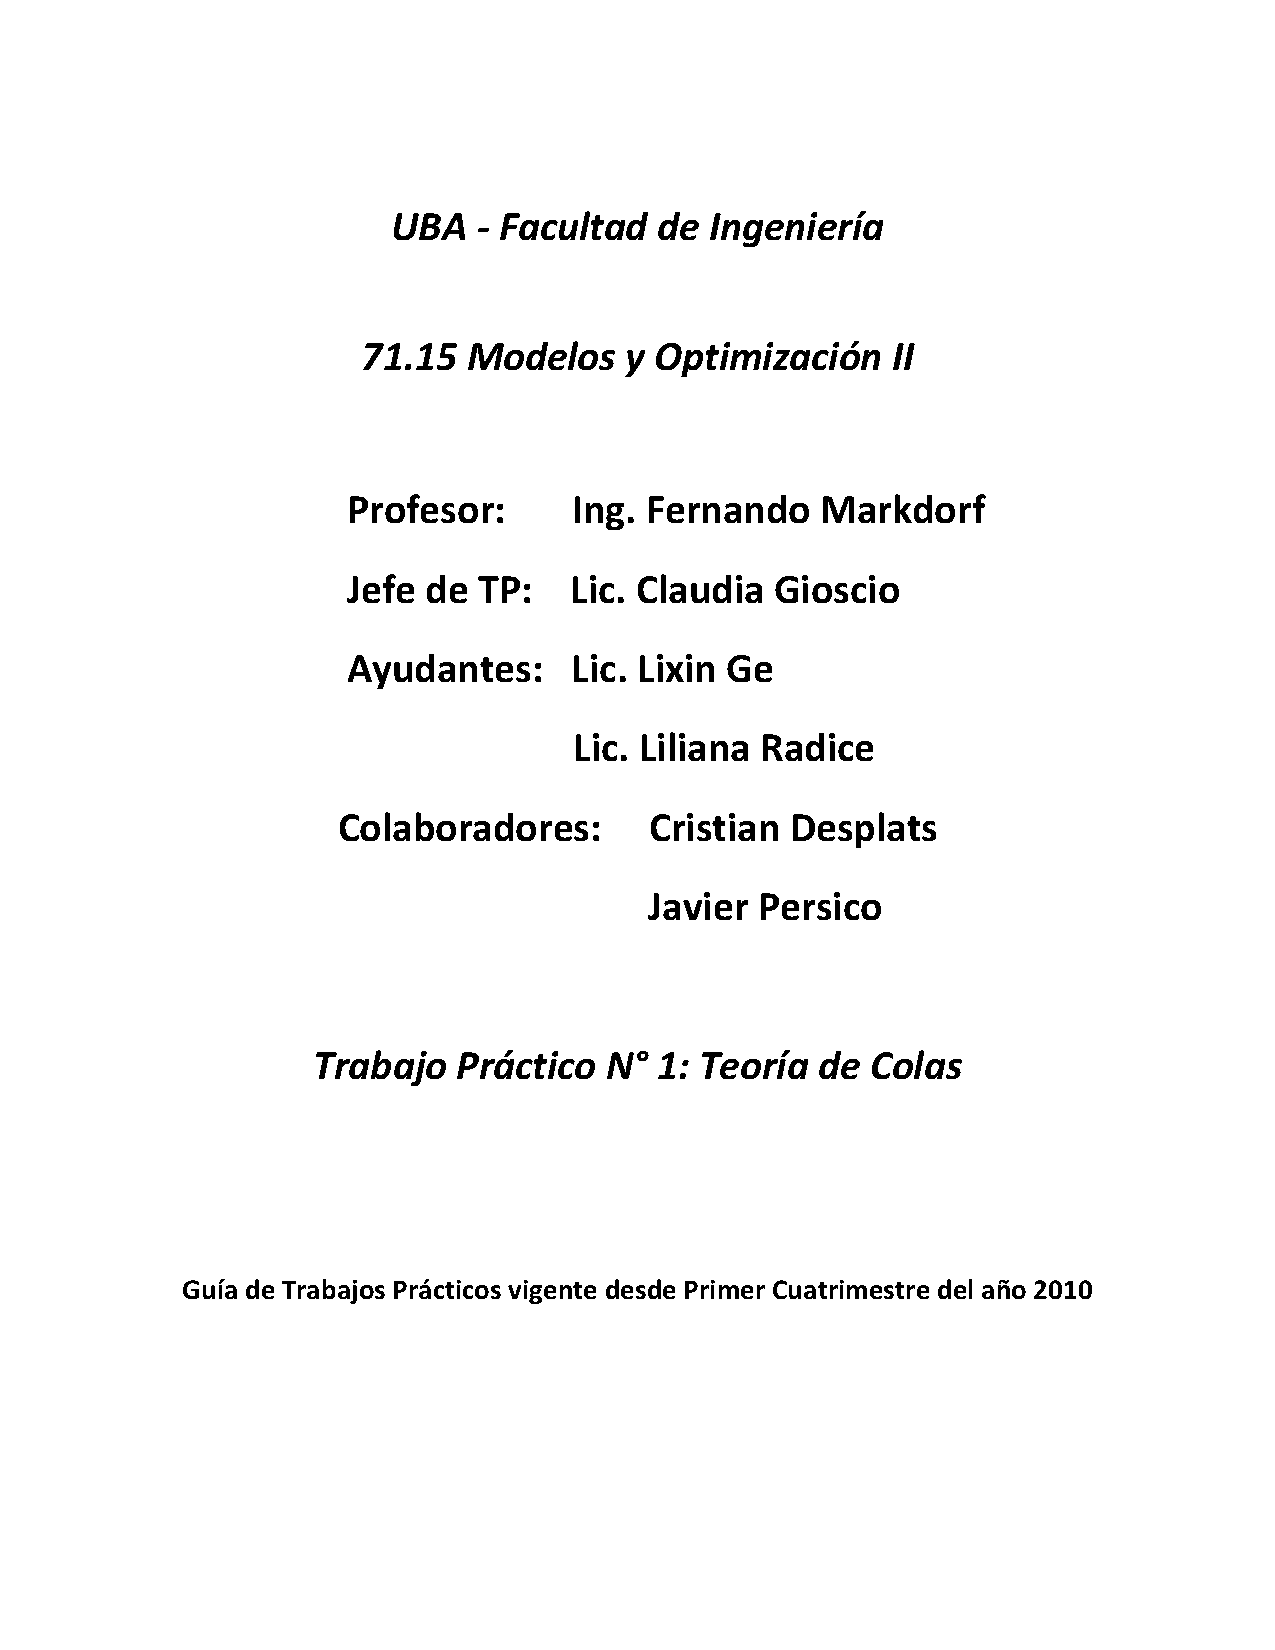
\includepdf[pages={-}]{enunciado.pdf}

\clearpage
\end{document}
